\documentclass[border=0pt]{standalone}
% Source of docs/assets/arch_v3.png.
% Build: xelatex arch_v3.tex
%        pdftocairo -png -transp -r 300 -singlefile arch_v3.pdf arch_v3
% Feature-overview card: panels of pills, rounded sage card on a transparent background.
\usepackage{fontspec}
\usepackage{tikz}
\usetikzlibrary{arrows.meta, calc}

\setsansfont{Inter}[UprightFont={*-Regular}, BoldFont={*-SemiBold}, Ligatures=TeX]
\renewcommand{\familydefault}{\sfdefault}

\definecolor{bg}{HTML}{E5EBD9}
\definecolor{panelfill}{HTML}{F4F7EC}
\definecolor{panelborder}{HTML}{C9D4BA}
\definecolor{ink}{HTML}{1F241A}
\definecolor{muted}{HTML}{6F7468}
\definecolor{pillblue}{HTML}{D0DAEF}
\definecolor{bluetext}{HTML}{27396F}
\definecolor{pillsage}{HTML}{D7E2C4}
\definecolor{sagetext}{HTML}{3B4F2A}
\definecolor{pillgrey}{HTML}{DFE2D8}
\definecolor{greytext}{HTML}{474D42}

\tikzset{
  pill/.style={rounded corners=0.05cm, minimum height=0.44cm, inner xsep=0.04cm, inner ysep=0pt, font=\fontsize{8}{9}\selectfont},
  bpill/.style={pill, fill=pillblue, text=bluetext},
  spill/.style={pill, fill=pillsage, text=sagetext},
  gpill/.style={pill, fill=pillgrey, text=greytext},
}

\newcommand{\panel}[4]{%
  \fill[panelfill, rounded corners=0.10cm] (#1,#2) rectangle (#3,#4);%
  \draw[panelborder, line width=0.5pt, rounded corners=0.10cm] (#1,#2) rectangle (#3,#4);%
}
\newcommand{\ptitle}[3]{%
  \node[text=ink] at (#1,#2) {\fontsize{9.5}{11}\selectfont\bfseries #3};%
}
\newcommand{\pillrow}[5]{%
  \foreach \it [count=\i] in {#5}{%
    \node[pill, #4, minimum width=\dimexpr#3cm-0.10cm\relax] at ({#2+(\i-0.5)*#3},#1) {\it};%
  }%
}

\begin{document}
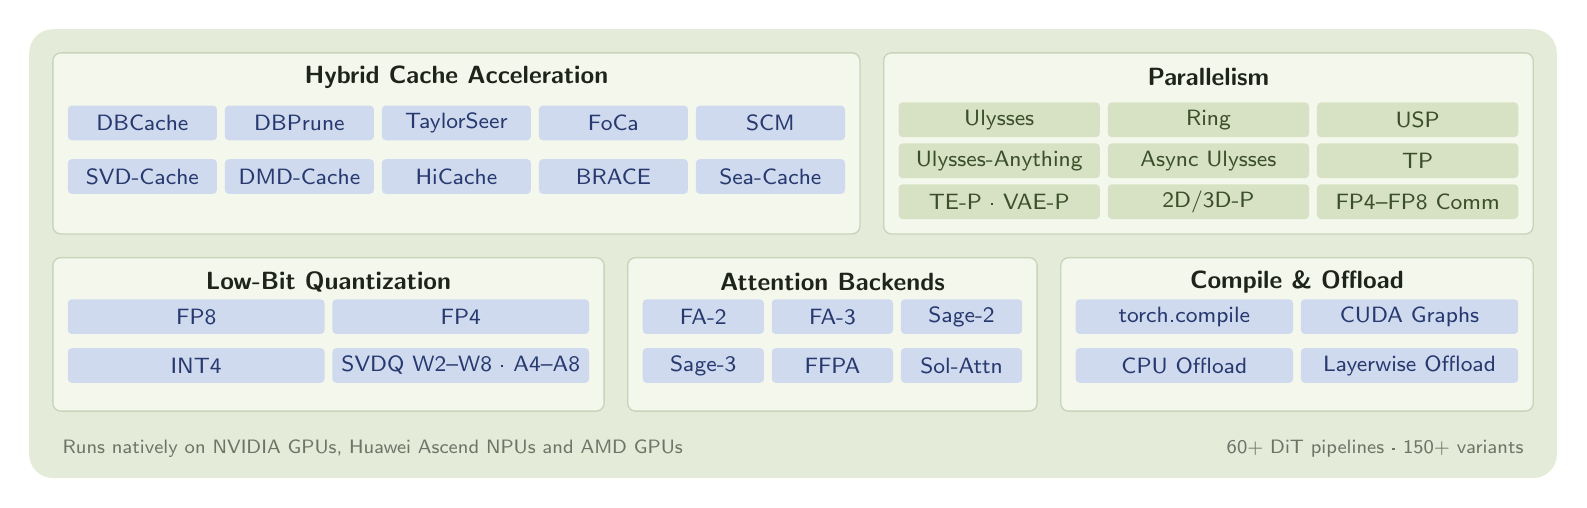
\begin{tikzpicture}[x=1cm, y=1cm]
  \path[use as bounding box] (-0.02,-0.02) rectangle (19.42,5.72);
  \fill[bg, rounded corners=0.30cm] (0,0) rectangle (19.40,5.70);

  \panel{0.30}{3.10}{10.55}{5.40}
  \ptitle{5.425}{5.09}{Hybrid Cache Acceleration}
  \pillrow{4.51}{0.44}{1.994}{bpill}{DBCache, DBPrune, TaylorSeer, FoCa, SCM}
  \pillrow{3.83}{0.44}{1.994}{bpill}{SVD-Cache, DMD-Cache, HiCache, BRACE, Sea-Cache}

  \panel{10.85}{3.10}{19.10}{5.40}
  \ptitle{14.975}{5.09}{Parallelism}
  \pillrow{4.55}{10.99}{2.657}{spill}{Ulysses, Ring, USP}
  \pillrow{4.03}{10.99}{2.657}{spill}{Ulysses-Anything, Async Ulysses, TP}
  \pillrow{3.51}{10.99}{2.657}{spill}{TE-P \textperiodcentered\ VAE-P, 2D/3D-P, FP4--FP8 Comm}

  \panel{0.30}{0.85}{7.30}{2.80}
  \ptitle{3.80}{2.49}{Low-Bit Quantization}
  \pillrow{2.05}{0.44}{3.36}{bpill}{FP8, FP4}
  \pillrow{1.43}{0.44}{3.36}{bpill}{INT4, SVDQ W2--W8 \textperiodcentered\ A4--A8}

  \panel{7.60}{0.85}{12.80}{2.80}
  \ptitle{10.20}{2.49}{Attention Backends}
  \pillrow{2.05}{7.74}{1.64}{bpill}{FA-2, FA-3, Sage-2}
  \pillrow{1.43}{7.74}{1.64}{bpill}{Sage-3, FFPA, Sol-Attn}

  \panel{13.10}{0.85}{19.10}{2.80}
  \ptitle{16.10}{2.49}{Compile \& Offload}
  \pillrow{2.05}{13.24}{2.86}{bpill}{torch.compile, CUDA Graphs}
  \pillrow{1.43}{13.24}{2.86}{bpill}{CPU Offload, Layerwise Offload}

  \node[anchor=west, text=muted] at (0.30,0.37) {\fontsize{7.5}{9}\selectfont Runs natively on NVIDIA GPUs, Huawei Ascend NPUs and AMD GPUs};
  \node[anchor=east, text=muted] at (19.10,0.37) {\fontsize{7.5}{9}\selectfont 60+ DiT pipelines \textperiodcentered\ 150+ variants};

\end{tikzpicture}
\end{document}
